\documentclass{article}
\usepackage[utf8]{inputenc}
\usepackage{amsmath}
\usepackage{amsthm}
\usepackage{bm}
\usepackage{amsfonts}
\usepackage{titlesec}
\usepackage{hyperref}
\usepackage{color}
\usepackage{booktabs}
\usepackage{amsthm}
\usepackage{listings}
\usepackage{exsheets}

%% Font Policy
% vector, \bm{}
% matrix, \bm{}
% space, \mathbb{}

%%%% Define "Lecture" (from redefining "Chapter") %%%% 
% \titleformat{\chapter}[block]{\LARGE\bfseries}{Lecture~\arabic{chapter}.}{1em}{}[]
%%%% ============================================ %%%%

%%% Set up exercise-solution format %%%
%\SetupExSheets{
	%	counter-format = ch.qu ,
	%	counter-within = chapter
	%}
%%% =============================== %%%

\renewcommand{\vec}[1]{\bm{#1}}
\newtheorem*{remark}{Remark}
\newtheorem{theorem}{Theorem}[section]
\newtheorem{definition}{Definition}[section]
\newtheorem{problem}{Problem}
\newtheorem{corollary}{Corollary}[section]
\newtheorem{lemma}{Lemma}[section]
\newtheorem{property}{Property}[section]

\author{Fang Zhu}
\title{Lecture 6 Projectors}

\begin{document}
	\maketitle
	
\section{Prerequisite}


\section{Solutions}
\subsection{Exercise 6.1}
\begin{proof}
    Since $\bm{P}$ is an orthogonal projector, then we have $\bm{P}^2 = \bm{P}$ and $\bm{P}^{\star} = \bm{P}$, hence 
    \begin{equation}
        (\bm{I} - 2\bm{P})^{\star}  (\bm{I} - 2\bm{P}) = \bm{I} - 2\bm{P}^\star - 2 \bm{P} + 4 \bm{P}^\star \bm{P} = 0,
    \end{equation}
    which means that $\bm{I} - 2 \bm{P}$ is unitary. A geometric interpretation is given by \autoref{fig:geo_e61}.
    \begin{figure}[htpb]
        \centering
        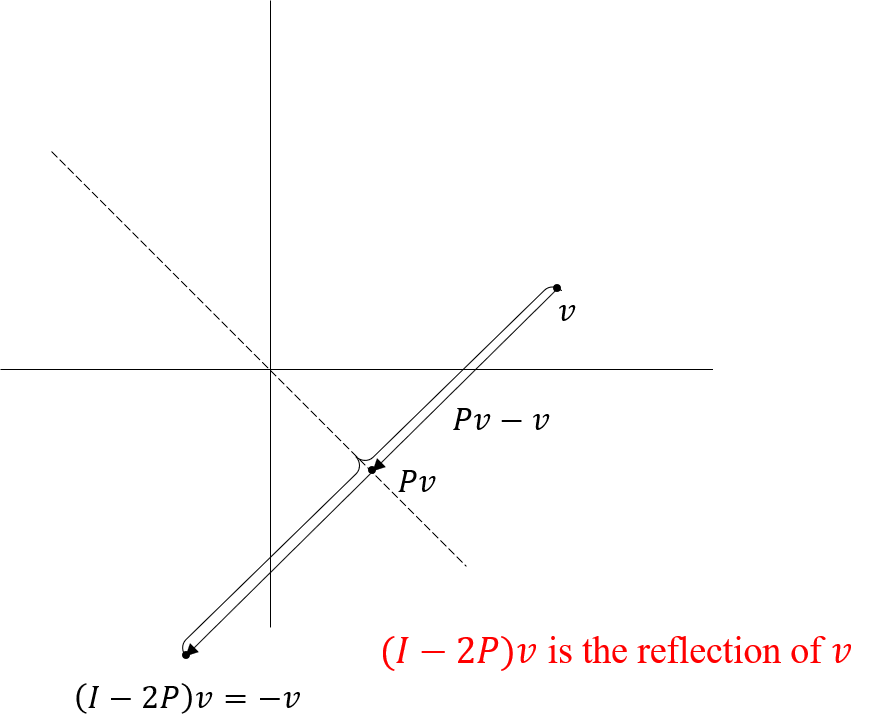
\includegraphics[width=0.5\textwidth]{e61.png}
        \caption{Geometric interpretation of $\bm{I} - 2\bm{P}$.}
        \label{fig:geo_e61}
    \end{figure}
\end{proof}

\end{document}